% Topic T1.2: Financial System's Pain Points
% Self-contained Beamer slides for Digital Finance course
\documentclass[11pt,aspectratio=169]{beamer}
\usetheme{Madrid}

% ======================= PACKAGES =======================
\usepackage{graphicx}
\usepackage{booktabs}
\usepackage{adjustbox}
\usepackage{multicol}
\usepackage{amsmath}
\usepackage{amssymb}
\usepackage{tikz}
\usetikzlibrary{arrows,shapes,positioning,shadows,trees}
\usepackage{listings}
\usepackage{xcolor}

% ======================= COLOR DEFINITIONS =======================
% Primary color scheme: Blue/Teal for Digital Finance
\definecolor{dfblue}{RGB}{0,102,204}
\definecolor{dfteal}{RGB}{0,153,153}
\definecolor{dfcyan}{RGB}{51,187,204}
\definecolor{dflightblue}{RGB}{153,204,255}
\definecolor{dflightblue2}{RGB}{173,214,255}
\definecolor{dflightblue3}{RGB}{193,224,255}
\definecolor{dflightblue4}{RGB}{213,234,255}

% Accent colors for finance applications
\definecolor{dfgreen}{RGB}{44, 160, 44}
\definecolor{dfred}{RGB}{214, 39, 40}
\definecolor{dforange}{RGB}{255, 127, 14}
\definecolor{dfgray}{RGB}{127, 127, 127}

% Utility colors
\definecolor{lightgray}{RGB}{240, 240, 240}
\definecolor{midgray}{RGB}{180, 180, 180}
\definecolor{codebg}{RGB}{245, 245, 245}

% ======================= THEME CUSTOMIZATION =======================
% Apply Digital Finance color scheme to Madrid theme
\setbeamercolor{palette primary}{bg=dflightblue3,fg=dfblue}
\setbeamercolor{palette secondary}{bg=dflightblue2,fg=dfblue}
\setbeamercolor{palette tertiary}{bg=dfteal,fg=white}
\setbeamercolor{palette quaternary}{bg=dfblue,fg=white}

\setbeamercolor{structure}{fg=dfblue}
\setbeamercolor{section in toc}{fg=dfblue}
\setbeamercolor{subsection in toc}{fg=dfteal}
\setbeamercolor{title}{fg=dfblue}
\setbeamercolor{frametitle}{fg=dfblue,bg=dflightblue3}
\setbeamercolor{block title}{bg=dflightblue2,fg=dfblue}
\setbeamercolor{block body}{bg=dflightblue4,fg=black}

% Remove navigation symbols for cleaner look
\setbeamertemplate{navigation symbols}{}

% Clean itemize/enumerate
\setbeamertemplate{itemize items}[circle]
\setbeamertemplate{enumerate items}[default]

% Margins for readability
\setbeamersize{text margin left=8mm,text margin right=8mm}

% ======================= LISTINGS CONFIGURATION =======================
% Python code style
\lstdefinestyle{pythonstyle}{
    language=Python,
    basicstyle=\ttfamily\footnotesize,
    keywordstyle=\color{dfblue}\bfseries,
    stringstyle=\color{dforange},
    commentstyle=\color{dfgray}\itshape,
    numberstyle=\tiny\color{dfgray},
    numbers=left,
    numbersep=5pt,
    backgroundcolor=\color{codebg},
    showspaces=false,
    showstringspaces=false,
    showtabs=false,
    frame=single,
    rulecolor=\color{midgray},
    tabsize=4,
    captionpos=b,
    breaklines=true,
    breakatwhitespace=false,
    escapeinside={(*@}{@*)},
    xleftmargin=10pt,
    xrightmargin=10pt
}

% Solidity code style
\lstdefinestyle{soliditystyle}{
    language=Java, % closest approximation
    basicstyle=\ttfamily\footnotesize,
    keywordstyle=\color{dfteal}\bfseries,
    stringstyle=\color{dforange},
    commentstyle=\color{dfgray}\itshape,
    numberstyle=\tiny\color{dfgray},
    numbers=left,
    numbersep=5pt,
    backgroundcolor=\color{codebg},
    showspaces=false,
    showstringspaces=false,
    showtabs=false,
    frame=single,
    rulecolor=\color{midgray},
    tabsize=2,
    captionpos=b,
    breaklines=true,
    breakatwhitespace=false,
    escapeinside={(*@}{@*)},
    xleftmargin=10pt,
    xrightmargin=10pt,
    morekeywords={pragma, contract, function, returns, public, private, view, pure, payable, address, uint256, mapping, event, modifier}
}

% Inline code command
\newcommand{\code}[1]{\texttt{\color{dfblue}#1}}

% ======================= CUSTOM COMMANDS =======================
% Bottom annotation (Madrid-style)
\newcommand{\bottomnote}[1]{%
\vfill
\vspace{-2mm}
\textcolor{dflightblue2}{\rule{\textwidth}{0.4pt}}
\vspace{1mm}
\footnotesize
\textbf{#1}
}

% Compact list spacing
\newcommand{\compactlist}{%
\setlength{\itemsep}{0pt}%
\setlength{\parskip}{0pt}%
\setlength{\parsep}{0pt}%
}

% Chart placeholder
\newcommand{\chartplaceholder}[2][5cm]{%
\begin{center}
\begin{adjustbox}{max width=0.95\textwidth, max height=#1}
\framebox[\textwidth][c]{%
\rule{0pt}{#1}%
\textcolor{midgray}{[#2]}%
}
\end{adjustbox}
\end{center}
}

% ======================= FINANCE NOTATION MACROS =======================
% Probability and statistics
\newcommand{\E}{\mathbb{E}} % Expected value
\newcommand{\Var}{\mathrm{Var}} % Variance
\newcommand{\Cov}{\mathrm{Cov}} % Covariance
\newcommand{\Prob}{\mathbb{P}} % Probability

% Distributions
\newcommand{\Normal}{\mathcal{N}} % Normal distribution
\newcommand{\Uniform}{\mathcal{U}} % Uniform distribution

% Returns and prices
\newcommand{\Ret}{R} % Return
\newcommand{\LogRet}{r} % Log return
\newcommand{\Price}{S} % Price/Stock price
\newcommand{\Strike}{K} % Strike price

% Options and derivatives
\newcommand{\CallPrice}{C} % Call option price
\newcommand{\PutPrice}{P} % Put option price
\newcommand{\Greeks}[1]{\mathit{#1}} % Greek letters

% Risk measures
\newcommand{\VaR}{\mathrm{VaR}} % Value at Risk
\newcommand{\CVaR}{\mathrm{CVaR}} % Conditional VaR
\newcommand{\Sharpe}{\mathrm{SR}} % Sharpe Ratio

% Time series
\newcommand{\AR}{\mathrm{AR}} % Autoregressive
\newcommand{\MA}{\mathrm{MA}} % Moving average
\newcommand{\GARCH}{\mathrm{GARCH}} % GARCH

% Blockchain/Crypto
\newcommand{\Hash}{\mathrm{Hash}} % Hash function
\newcommand{\Block}{\mathcal{B}} % Block
\newcommand{\Chain}{\mathcal{C}} % Chain

% Real numbers, integers
\newcommand{\R}{\mathbb{R}}
\newcommand{\Z}{\mathbb{Z}}
\newcommand{\N}{\mathbb{N}}

% ======================= TIKZ STYLES =======================
% Styles for finance-related diagrams
\tikzstyle{process} = [rectangle, minimum width=3cm, minimum height=1cm, text centered, draw=dfblue, fill=dflightblue4, thick]
\tikzstyle{decision} = [diamond, minimum width=3cm, minimum height=1cm, text centered, draw=dfteal, fill=dflightblue4, thick]
\tikzstyle{arrow} = [thick,->,>=stealth,color=dfblue]
\tikzstyle{blockchain} = [rectangle, rounded corners, minimum width=2.5cm, minimum height=1cm, text centered, draw=dfteal, fill=dflightblue3, thick]
\tikzstyle{transaction} = [circle, minimum size=0.8cm, text centered, draw=dforange, fill=dflightblue4, thick]

% ======================= FOOTER TEMPLATE =======================
\setbeamertemplate{footline}{
    \hbox{\begin{beamercolorbox}[wd=\paperwidth,ht=2.5ex,dp=1ex,leftskip=.5em,rightskip=.5em]{author in head/foot}
    \tiny
    \textbf{Digital Finance} \hfill
    Joerg Osterrieder \hfill
    \insertdate \hfill
    Page \insertframenumber{} / \inserttotalframenumber
    \end{beamercolorbox}}
}

% ======================= SECTION DIVIDER TEMPLATE =======================
\AtBeginSection[]{
\begin{frame}[plain]
\vfill
\centering
\begin{beamercolorbox}[sep=12pt,center]{title}
\usebeamerfont{title}\LARGE\insertsection\par
\end{beamercolorbox}
\vfill
\end{frame}
}


\title[T1.2: Pain Points]{Topic 1.2: Financial System's Pain Points}
\subtitle{Where Friction Creates Opportunity}
\author{Joerg Osterrieder}
\institute{Digital Finance}
\date{2025}

\begin{document}

%--- Frame 1: Title ---
\begin{frame}
\titlepage
\end{frame}

%--- Frame 2: Learning Objectives ---
\begin{frame}{Learning Objectives}
\begin{block}{By the end of this topic, you will be able to:}
\begin{enumerate}
\item \textbf{Identify} the 6 core frictions in traditional finance systems
\item \textbf{Understand} who bears the cost of each friction and how
\item \textbf{Analyze} why these frictions persist despite technological advances
\item \textbf{Connect} each friction to digital finance innovations that address it
\item \textbf{Evaluate} which frictions cause the most societal harm
\end{enumerate}
\end{block}

\vspace{5mm}
\begin{alertblock}{Key Insight}
Every FinTech and DeFi innovation targets a specific friction. Understanding the frictions helps you understand the solutions.
\end{alertblock}
\end{frame}

%--- Frame 3: Prerequisites ---
\begin{frame}{Prerequisites and Background}
\begin{columns}[T]
\begin{column}{0.48\textwidth}
\textbf{What You Should Know:}
\begin{itemize}
\item Basic understanding of how banks operate
\item Familiarity with common payment methods
\item Awareness of international money transfers
\item General knowledge of stock market trading
\end{itemize}
\end{column}
\begin{column}{0.48\textwidth}
\textbf{Building On Topic 1.1:}
\begin{itemize}
\item The financial system serves critical functions
\item Multiple intermediaries exist for historical reasons
\item Trust is distributed across institutions
\item Regulation shapes system structure
\end{itemize}
\end{column}
\end{columns}

\vspace{5mm}
\begin{block}{Connection to Course}
Understanding pain points is essential for evaluating whether digital finance solutions actually solve real problems or create new ones.
\end{block}
\end{frame}

%--- Frame 4: The Big Picture ---
\begin{frame}{The Big Picture: Why Study Pain Points?}
\begin{center}
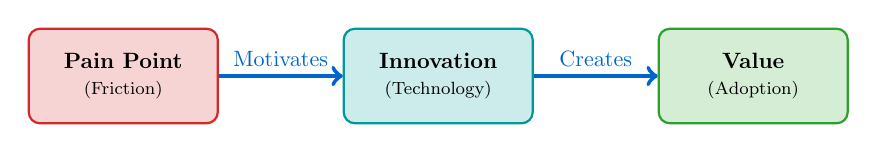
\begin{tikzpicture}[scale=0.8, transform shape]
% Three connected boxes
\node (problem) [blockchain, minimum width=3cm, minimum height=1.5cm, fill=dfred!20, draw=dfred] {
\begin{tabular}{c}
\textbf{Pain Point}\\
\footnotesize (Friction)
\end{tabular}
};

\node (innovation) [blockchain, right of=problem, node distance=5cm, minimum width=3cm, minimum height=1.5cm, fill=dfteal!20, draw=dfteal] {
\begin{tabular}{c}
\textbf{Innovation}\\
\footnotesize (Technology)
\end{tabular}
};

\node (value) [blockchain, right of=innovation, node distance=5cm, minimum width=3cm, minimum height=1.5cm, fill=dfgreen!20, draw=dfgreen] {
\begin{tabular}{c}
\textbf{Value}\\
\footnotesize (Adoption)
\end{tabular}
};

\draw[->, ultra thick, dfblue] (problem) -- node[above] {Motivates} (innovation);
\draw[->, ultra thick, dfblue] (innovation) -- node[above] {Creates} (value);
\end{tikzpicture}
\end{center}

\vspace{5mm}
\textbf{Framework for Analysis:}
\begin{itemize}
\item Innovations that don't address real pain points fail
\item The bigger the friction, the bigger the opportunity
\item Friction = value captured by intermediaries (or lost entirely)
\end{itemize}
\end{frame}

%--- Frame 5: The Global Financial System ---
\begin{frame}{The Global Financial System: A Marvel of Complexity}
\begin{center}
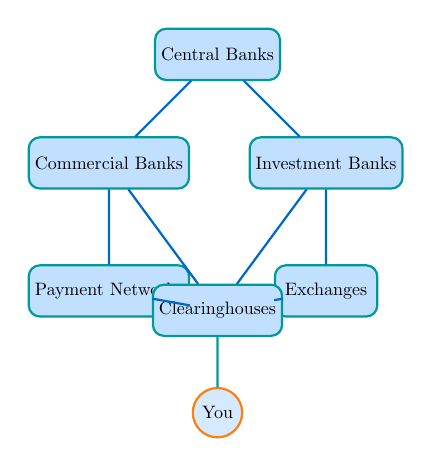
\begin{tikzpicture}[scale=0.65, transform shape]
% Central banks
\node (fed) [blockchain, minimum width=2cm] {Central Banks};
\node (comm) [blockchain, below left of=fed, node distance=3cm, minimum width=2cm] {Commercial Banks};
\node (inv) [blockchain, below right of=fed, node distance=3cm, minimum width=2cm] {Investment Banks};
\node (pay) [blockchain, below of=comm, node distance=2.5cm, minimum width=2cm] {Payment Networks};
\node (exch) [blockchain, below of=inv, node distance=2.5cm, minimum width=2cm] {Exchanges};
\node (clear) [blockchain, below of=fed, node distance=5cm, minimum width=2cm] {Clearinghouses};

% Connections
\draw[thick, dfblue] (fed) -- (comm);
\draw[thick, dfblue] (fed) -- (inv);
\draw[thick, dfblue] (comm) -- (pay);
\draw[thick, dfblue] (inv) -- (exch);
\draw[thick, dfblue] (comm) -- (clear);
\draw[thick, dfblue] (inv) -- (clear);
\draw[thick, dfblue] (pay) -- (clear);
\draw[thick, dfblue] (exch) -- (clear);

% Users
\node (user) [transaction, below of=clear, node distance=2cm] {You};
\draw[thick, dfteal] (user) -- (clear);
\end{tikzpicture}
\end{center}

\footnotesize
This system moves \textbf{\$9.6 trillion daily}, serves billions, rarely fails catastrophically... but has significant frictions.
\end{frame}

%--- Frame 6: Overview of the Six Frictions ---
\begin{frame}{The Six Frictions: Overview}
\begin{center}
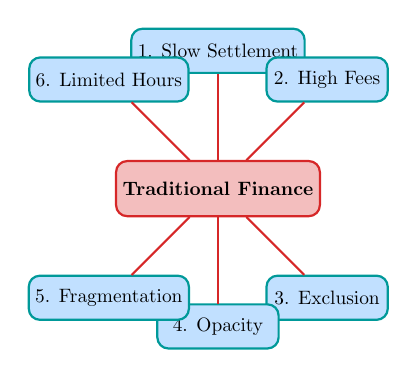
\begin{tikzpicture}[scale=0.7, transform shape]
% Central node
\node (center) [blockchain, minimum width=2.5cm, fill=dfred!30, draw=dfred] {\textbf{Traditional Finance}};

% Six frictions around it
\node (f1) [blockchain, above of=center, node distance=2.5cm, minimum width=2.2cm, minimum height=0.8cm] {1. Slow Settlement};
\node (f2) [blockchain, above right of=center, node distance=2.8cm, minimum width=2.2cm, minimum height=0.8cm] {2. High Fees};
\node (f3) [blockchain, below right of=center, node distance=2.8cm, minimum width=2.2cm, minimum height=0.8cm] {3. Exclusion};
\node (f4) [blockchain, below of=center, node distance=2.5cm, minimum width=2.2cm, minimum height=0.8cm] {4. Opacity};
\node (f5) [blockchain, below left of=center, node distance=2.8cm, minimum width=2.2cm, minimum height=0.8cm] {5. Fragmentation};
\node (f6) [blockchain, above left of=center, node distance=2.8cm, minimum width=2.2cm, minimum height=0.8cm] {6. Limited Hours};

% Connections
\draw[thick, dfred] (center) -- (f1);
\draw[thick, dfred] (center) -- (f2);
\draw[thick, dfred] (center) -- (f3);
\draw[thick, dfred] (center) -- (f4);
\draw[thick, dfred] (center) -- (f5);
\draw[thick, dfred] (center) -- (f6);
\end{tikzpicture}
\end{center}

\vspace{3mm}
Each friction represents billions of dollars in costs and millions of people affected.
\end{frame}

%--- Frame 7: Friction #1 - Slow Settlement (Overview) ---
\begin{frame}{Friction \#1: Slow Settlement}
\begin{columns}[T]
\begin{column}{0.55\textwidth}
\textbf{The Problem:}
\begin{itemize}
\item Stock trade: T+1 (1 business day since May 2024)
\item International wire: 1-5 business days
\item ACH transfer: 2-3 business days
\item Even ``instant'' payments take hours behind scenes
\end{itemize}

\vspace{3mm}
\textbf{Why so slow?}
\begin{itemize}
\item Multiple intermediaries
\item Batch processing (not real-time)
\item Timezone differences
\item Manual compliance checks
\item Legacy systems from 1970s
\end{itemize}
\end{column}
\begin{column}{0.42\textwidth}
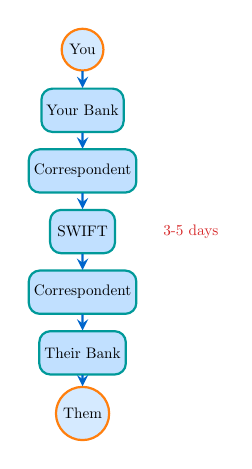
\begin{tikzpicture}[scale=0.55, transform shape, node distance=1.4cm]
% Settlement chain
\node (you) [transaction] {You};
\node (bank1) [blockchain, below of=you, minimum width=1.5cm] {Your Bank};
\node (corr1) [blockchain, below of=bank1, minimum width=1.5cm] {Correspondent};
\node (swift) [blockchain, below of=corr1, minimum width=1.5cm] {SWIFT};
\node (corr2) [blockchain, below of=swift, minimum width=1.5cm] {Correspondent};
\node (bank2) [blockchain, below of=corr2, minimum width=1.5cm] {Their Bank};
\node (them) [transaction, below of=bank2] {Them};

\draw[arrow] (you) -- (bank1);
\draw[arrow] (bank1) -- (corr1);
\draw[arrow] (corr1) -- (swift);
\draw[arrow] (swift) -- (corr2);
\draw[arrow] (corr2) -- (bank2);
\draw[arrow] (bank2) -- (them);

\node[right of=swift, node distance=2.5cm] {\textcolor{dfred}{3-5 days}};
\end{tikzpicture}
\end{column}
\end{columns}
\end{frame}

%--- Frame 8: Slow Settlement - Deep Dive ---
\begin{frame}{Slow Settlement: The Technical Reality}
\begin{columns}[T]
\begin{column}{0.5\textwidth}
\textbf{Batch Processing Explained:}
\begin{itemize}
\item Transactions queue during the day
\item Processed in batches overnight
\item ACH runs 4-5 times per day
\item Fedwire: real-time but expensive
\item SWIFT: messaging only, not settlement
\end{itemize}

\vspace{3mm}
\textbf{The T+1 Journey:}
\begin{enumerate}
\item Trade execution (instant)
\item Trade confirmation (hours)
\item Clearing (overnight)
\item Settlement (next day)
\end{enumerate}
\end{column}
\begin{column}{0.48\textwidth}
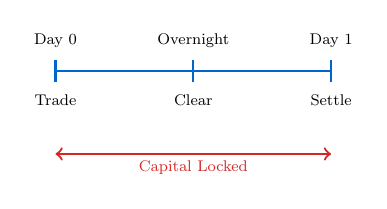
\begin{tikzpicture}[scale=0.7, transform shape]
% Timeline
\draw[thick, dfblue] (0,0) -- (5,0);
\draw[thick, dfblue] (0,-0.2) -- (0,0.2);
\draw[thick, dfblue] (2.5,-0.2) -- (2.5,0.2);
\draw[thick, dfblue] (5,-0.2) -- (5,0.2);

\node[above] at (0,0.3) {\footnotesize Day 0};
\node[above] at (2.5,0.3) {\footnotesize Overnight};
\node[above] at (5,0.3) {\footnotesize Day 1};

\node[below] at (0,-0.3) {\footnotesize Trade};
\node[below] at (2.5,-0.3) {\footnotesize Clear};
\node[below] at (5,-0.3) {\footnotesize Settle};

% Capital locked
\draw[thick, dfred, <->] (0,-1.5) -- (5,-1.5);
\node[below, dfred] at (2.5,-1.5) {\footnotesize Capital Locked};
\end{tikzpicture}

\vspace{5mm}
\begin{alertblock}{Cost Impact}
\$1 trillion locked in settlement = \$50M+/day in opportunity cost (at 2\% annual rate)
\end{alertblock}
\end{column}
\end{columns}
\end{frame}

%--- Frame 9: Slow Settlement - Consequences ---
\begin{frame}{Slow Settlement: Who Pays?}
\textbf{Direct Costs of Settlement Delays:}

\begin{center}
\renewcommand{\arraystretch}{1.3}
\begin{tabular}{|l|l|p{5.5cm}|}
\hline
\textbf{Stakeholder} & \textbf{Cost Type} & \textbf{Impact} \\
\hline
Businesses & Working capital & Cannot use funds for 1-5 days \\
\hline
Traders & Counterparty risk & Exposure until settlement \\
\hline
Banks & Capital requirements & Must hold reserves for pending trades \\
\hline
Consumers & Opportunity cost & Money in transit earns nothing \\
\hline
Markets & Systemic risk & Failure cascades during crisis \\
\hline
\end{tabular}
\end{center}

\vspace{3mm}
\begin{block}{2008 Financial Crisis Connection}
Lehman Brothers' failure created \$600B+ in unsettled trades. Settlement delay amplified contagion risk across the entire financial system.
\end{block}
\end{frame}

%--- Frame 10: Friction #2 - High Fees (Overview) ---
\begin{frame}{Friction \#2: High Fees (Especially Cross-Border)}
\begin{center}
\textbf{Cost of Sending \$200 Internationally}
\end{center}

\begin{center}
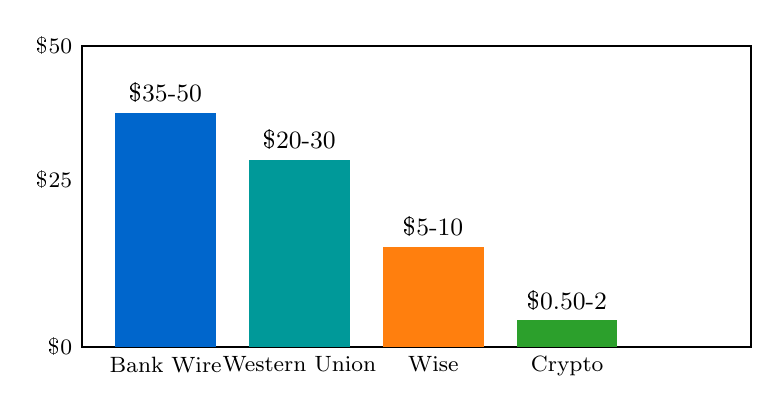
\begin{tikzpicture}[scale=0.85]
% Bar chart
\draw[thick] (0,0) -- (10,0) -- (10,4.5) -- (0,4.5) -- cycle;

% Bars
\fill[dfblue] (0.5,0) rectangle (2,3.5);
\fill[dfteal] (2.5,0) rectangle (4,2.8);
\fill[dforange] (4.5,0) rectangle (6,1.5);
\fill[dfgreen] (6.5,0) rectangle (8,0.4);

% Labels
\node[below, font=\footnotesize] at (1.25,0) {Bank Wire};
\node[below, font=\footnotesize] at (3.25,0) {Western Union};
\node[below, font=\footnotesize] at (5.25,0) {Wise};
\node[below, font=\footnotesize] at (7.25,0) {Crypto};

% Values
\node[above, font=\small] at (1.25,3.5) {\$35-50};
\node[above, font=\small] at (3.25,2.8) {\$20-30};
\node[above, font=\small] at (5.25,1.5) {\$5-10};
\node[above, font=\small] at (7.25,0.4) {\$0.50-2};

% Y-axis
\node[left] at (0,0) {\footnotesize \$0};
\node[left] at (0,2.5) {\footnotesize \$25};
\node[left] at (0,4.5) {\footnotesize \$50};
\end{tikzpicture}
\end{center}

\vspace{3mm}
\textbf{Who pays?} Migrant workers sending money home. The global remittance market is \textbf{\$700+ billion/year}, with \textbf{\$50+ billion} lost to fees.
\end{frame}

%--- Frame 11: High Fees - Fee Breakdown ---
\begin{frame}{High Fees: Where Does Your Money Go?}
\begin{columns}[T]
\begin{column}{0.5\textwidth}
\textbf{Components of a \$50 Wire Fee:}
\begin{itemize}
\item Originating bank fee: \$15-25
\item SWIFT messaging: \$3-5
\item Correspondent bank(s): \$10-20
\item Receiving bank fee: \$5-15
\item FX spread (hidden): 2-4\%
\end{itemize}

\vspace{3mm}
\textbf{Hidden Costs:}
\begin{itemize}
\item Exchange rate markup
\item Intermediary deductions
\item ``Lifting fees''
\item Delay costs
\end{itemize}
\end{column}
\begin{column}{0.48\textwidth}
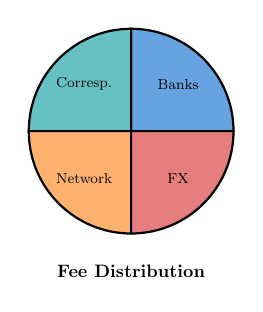
\begin{tikzpicture}[scale=0.65, transform shape]
% Pie chart representation
\draw[thick, fill=dfblue!60] (0,0) -- (0:2) arc (0:90:2) -- cycle;
\draw[thick, fill=dfteal!60] (0,0) -- (90:2) arc (90:180:2) -- cycle;
\draw[thick, fill=dforange!60] (0,0) -- (180:2) arc (180:270:2) -- cycle;
\draw[thick, fill=dfred!60] (0,0) -- (270:2) arc (270:360:2) -- cycle;

% Labels
\node at (45:1.3) {\footnotesize Banks};
\node at (135:1.3) {\footnotesize Corresp.};
\node at (225:1.3) {\footnotesize Network};
\node at (315:1.3) {\footnotesize FX};

\node[below] at (0,-2.5) {\textbf{Fee Distribution}};
\end{tikzpicture}

\vspace{3mm}
\footnotesize
\textbf{Result:} A \$200 remittance can cost 10-15\% in total fees when all costs are included.
\end{column}
\end{columns}
\end{frame}

%--- Frame 12: High Fees - Global Impact ---
\begin{frame}{High Fees: The Human Cost}
\begin{center}
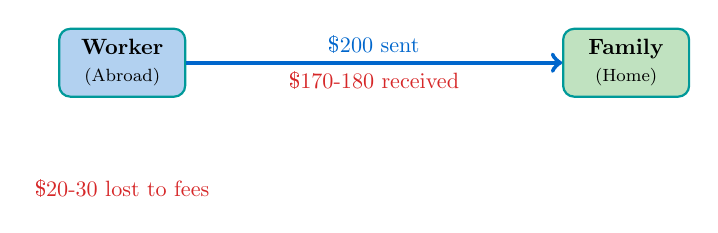
\begin{tikzpicture}[scale=0.8, transform shape]
% World map simplified representation
\node (origin) [blockchain, minimum width=2cm, fill=dfblue!30] {
\begin{tabular}{c}
\textbf{Worker}\\
\footnotesize (Abroad)
\end{tabular}
};

\node (dest) [blockchain, right of=origin, node distance=8cm, minimum width=2cm, fill=dfgreen!30] {
\begin{tabular}{c}
\textbf{Family}\\
\footnotesize (Home)
\end{tabular}
};

% Money flow
\draw[->, ultra thick, dfblue] (origin) -- node[above] {\$200 sent} node[below] {\textcolor{dfred}{\$170-180 received}} (dest);

% Leakage
\node[below of=origin, node distance=2cm, dfred] {\$20-30 lost to fees};
\end{tikzpicture}
\end{center}

\vspace{3mm}
\textbf{Global Statistics:}
\begin{itemize}
\item \textbf{200+ million} migrant workers worldwide
\item Average remittance fee: \textbf{6.4\%} globally (2023)
\item Sub-Saharan Africa: \textbf{8-9\%} average fees
\item UN SDG target: reduce to \textbf{3\%} by 2030
\item \textbf{\$50+ billion/year} lost to fees that could lift millions from poverty
\end{itemize}
\end{frame}

%--- Frame 13: Friction #3 - Financial Exclusion ---
\begin{frame}{Friction \#3: Financial Exclusion}
\begin{columns}[T]
\begin{column}{0.5\textwidth}
\textbf{The Unbanked and Underbanked:}
\begin{itemize}
\item \textbf{1.4 billion} adults globally have no bank account
\item \textbf{Additional 1+ billion} are underbanked
\item In the US: 6\% unbanked, 18\% underbanked
\end{itemize}

\vspace{3mm}
\textbf{Why excluded?}
\begin{itemize}
\item No ID documents
\item No fixed address
\item Minimum balance requirements
\item Poor credit history
\item Geographic distance from banks
\item Distrust of institutions
\end{itemize}
\end{column}
\begin{column}{0.48\textwidth}
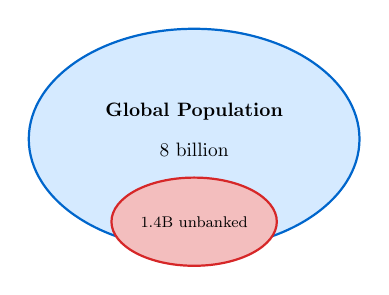
\begin{tikzpicture}[scale=0.7, transform shape]
% World map representation (simplified)
\draw[thick, dfblue, fill=dflightblue4] (0,0) ellipse (3cm and 2cm);
\node at (0,0.5) {\textbf{Global Population}};
\node at (0,-0.2) {8 billion};

% Excluded portion
\draw[thick, dfred, fill=dfred!30] (0,-1.5) ellipse (1.5cm and 0.8cm);
\node[font=\footnotesize] at (0,-1.5) {1.4B unbanked};
\end{tikzpicture}

\vspace{3mm}
\begin{alertblock}{The Paradox}
Those who need financial services most have the least access to them.
\end{alertblock}
\end{column}
\end{columns}
\end{frame}

%--- Frame 14: Financial Exclusion - Regional Breakdown ---
\begin{frame}{Financial Exclusion: Global Distribution}
\begin{center}
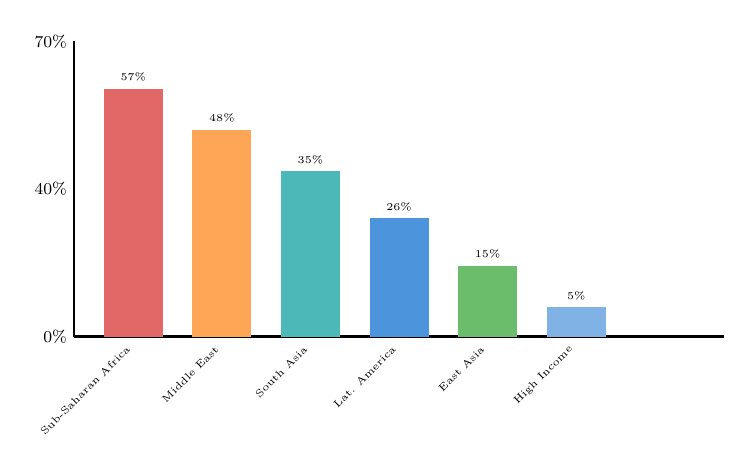
\begin{tikzpicture}[scale=0.75, transform shape]
% Bar chart - regional unbanked rates
\draw[thick] (0,0) -- (11,0);
\draw[thick] (0,0) -- (0,5);

% Bars
\fill[dfred!70] (0.5,0) rectangle (1.5,4.2);
\fill[dforange!70] (2,0) rectangle (3,3.5);
\fill[dfteal!70] (3.5,0) rectangle (4.5,2.8);
\fill[dfblue!70] (5,0) rectangle (6,2.0);
\fill[dfgreen!70] (6.5,0) rectangle (7.5,1.2);
\fill[dfblue!50] (8,0) rectangle (9,0.5);

% Labels
\node[below, font=\tiny, rotate=45, anchor=east] at (1,-0.1) {Sub-Saharan Africa};
\node[below, font=\tiny, rotate=45, anchor=east] at (2.5,-0.1) {Middle East};
\node[below, font=\tiny, rotate=45, anchor=east] at (4,-0.1) {South Asia};
\node[below, font=\tiny, rotate=45, anchor=east] at (5.5,-0.1) {Lat. America};
\node[below, font=\tiny, rotate=45, anchor=east] at (7,-0.1) {East Asia};
\node[below, font=\tiny, rotate=45, anchor=east] at (8.5,-0.1) {High Income};

% Values
\node[above, font=\tiny] at (1,4.2) {57\%};
\node[above, font=\tiny] at (2.5,3.5) {48\%};
\node[above, font=\tiny] at (4,2.8) {35\%};
\node[above, font=\tiny] at (5.5,2.0) {26\%};
\node[above, font=\tiny] at (7,1.2) {15\%};
\node[above, font=\tiny] at (8.5,0.5) {5\%};

% Y-axis
\node[left, font=\footnotesize] at (0,0) {0\%};
\node[left, font=\footnotesize] at (0,2.5) {40\%};
\node[left, font=\footnotesize] at (0,5) {70\%};
\end{tikzpicture}
\end{center}

\textbf{Key Insight:} Financial exclusion correlates with poverty, gender (women more excluded), rural location, and education level.
\end{frame}

%--- Frame 15: Financial Exclusion - Consequences ---
\begin{frame}{Financial Exclusion: The Cascading Effects}
\begin{center}
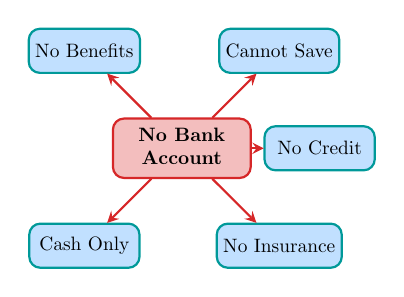
\begin{tikzpicture}[scale=0.7, transform shape, node distance=2.5cm]
% Central issue
\node (excl) [blockchain, minimum width=2.5cm, fill=dfred!30, draw=dfred] {
\begin{tabular}{c}
\textbf{No Bank}\\
\textbf{Account}
\end{tabular}
};

% Consequences
\node (save) [blockchain, above right of=excl, minimum width=2cm, minimum height=0.8cm] {Cannot Save};
\node (credit) [blockchain, right of=excl, minimum width=2cm, minimum height=0.8cm] {No Credit};
\node (insure) [blockchain, below right of=excl, minimum width=2cm, minimum height=0.8cm] {No Insurance};
\node (pay) [blockchain, below left of=excl, minimum width=2cm, minimum height=0.8cm] {Cash Only};
\node (govt) [blockchain, above left of=excl, minimum width=2cm, minimum height=0.8cm] {No Benefits};

\draw[arrow, dfred] (excl) -- (save);
\draw[arrow, dfred] (excl) -- (credit);
\draw[arrow, dfred] (excl) -- (insure);
\draw[arrow, dfred] (excl) -- (pay);
\draw[arrow, dfred] (excl) -- (govt);
\end{tikzpicture}
\end{center}

\vspace{3mm}
\textbf{Without financial access, people cannot:}
\begin{itemize}
\item Build savings for emergencies or education
\item Access credit to start businesses or buy homes
\item Insure against health, weather, or other risks
\item Receive government payments efficiently
\item Participate in the formal economy
\end{itemize}
\end{frame}

%--- Frame 16: Friction #4 - Opacity ---
\begin{frame}{Friction \#4: Opacity and Information Asymmetry}
\begin{columns}[T]
\begin{column}{0.55\textwidth}
\textbf{What you don't know:}
\begin{itemize}
\item True cost of financial products
\item Where your money goes
\item How prices are determined
\item What risks you're taking
\item How algorithms affect you
\end{itemize}

\vspace{3mm}
\textbf{Examples:}
\begin{itemize}
\item Hidden fees in mutual funds (expense ratios)
\item Payment for order flow in stock trading
\item Credit card interchange fees
\item Insurance pricing algorithms
\end{itemize}
\end{column}
\begin{column}{0.42\textwidth}
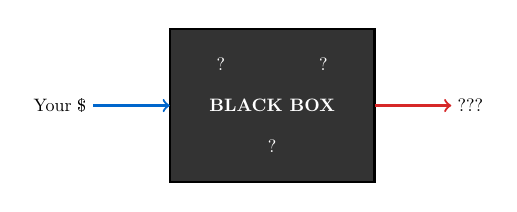
\begin{tikzpicture}[scale=0.65, transform shape]
% Black box
\draw[thick, fill=black!80] (0,0) rectangle (4,3);
\node[white] at (2,1.5) {\textbf{BLACK BOX}};

% Input
\draw[->, thick, dfblue] (-1.5,1.5) -- (0,1.5);
\node[left] at (-1.5,1.5) {Your \$};

% Output
\draw[->, thick, dfred] (4,1.5) -- (5.5,1.5);
\node[right] at (5.5,1.5) {???};

% Question marks
\node[white] at (1,2.3) {?};
\node[white] at (2,0.7) {?};
\node[white] at (3,2.3) {?};
\end{tikzpicture}

\vspace{5mm}
\footnotesize
\textbf{Information asymmetry} = one party knows more than the other. Usually favors financial institutions.
\end{column}
\end{columns}
\end{frame}

%--- Frame 17: Opacity - Real Examples ---
\begin{frame}{Opacity: Real-World Examples}
\begin{center}
\renewcommand{\arraystretch}{1.4}
\begin{tabular}{|p{3cm}|p{4cm}|p{4cm}|}
\hline
\textbf{Product} & \textbf{Hidden Element} & \textbf{Cost to Consumer} \\
\hline
Mutual Funds & Expense ratios, trading costs, soft dollars & 1-2\% annual drag on returns \\
\hline
Stock Trading & Payment for order flow (PFOF) & Worse execution prices \\
\hline
Credit Cards & Interchange fees (merchant pays) & Higher retail prices \\
\hline
Mortgages & Yield spread premiums, points & Thousands in extra interest \\
\hline
Insurance & Algorithmic pricing, risk factors & Unexplained premium differences \\
\hline
\end{tabular}
\end{center}

\begin{block}{The Asymmetry Problem}
Institutions have teams of analysts; consumers have Google. The information gap enables exploitation.
\end{block}
\end{frame}

%--- Frame 18: Opacity - Case Study: Payment for Order Flow ---
\begin{frame}{Opacity Case Study: Payment for Order Flow}
\begin{center}
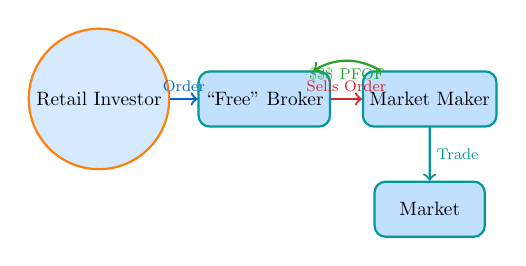
\begin{tikzpicture}[scale=0.7, transform shape, node distance=3cm]
% Actors
\node (retail) [transaction, minimum size=1cm] {Retail Investor};
\node (broker) [blockchain, right of=retail, minimum width=2.2cm] {``Free'' Broker};
\node (mm) [blockchain, right of=broker, minimum width=2.2cm] {Market Maker};

% Flows
\draw[->, thick, dfblue] (retail) -- node[above, font=\footnotesize] {Order} (broker);
\draw[->, thick, dfred] (broker) -- node[above, font=\footnotesize] {Sells Order} (mm);
\draw[->, thick, dfgreen] (mm) to[bend right=30] node[below, font=\footnotesize] {\$\$\$ PFOF} (broker);

% Market
\node (market) [blockchain, below of=mm, node distance=2cm, minimum width=2cm] {Market};
\draw[->, thick, dfteal] (mm) -- node[right, font=\footnotesize] {Trade} (market);
\end{tikzpicture}
\end{center}

\vspace{3mm}
\textbf{How it works:}
\begin{itemize}
\item Broker sells your orders to market makers
\item Market maker profits from spread (often pennies per share)
\item You may get slightly worse prices than the ``best'' available
\item ``Commission-free'' trading isn't actually free
\end{itemize}
\end{frame}

%--- Frame 19: Friction #5 - Fragmentation ---
\begin{frame}{Friction \#5: Fragmentation and Incompatibility}
\begin{center}
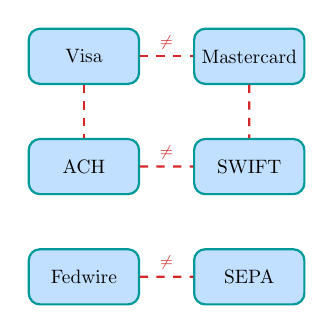
\begin{tikzpicture}[scale=0.7, transform shape]
% Different systems
\node (visa) [blockchain, minimum width=2cm] {Visa};
\node (mc) [blockchain, right of=visa, node distance=3cm, minimum width=2cm] {Mastercard};
\node (ach) [blockchain, below of=visa, node distance=2cm, minimum width=2cm] {ACH};
\node (swift) [blockchain, below of=mc, node distance=2cm, minimum width=2cm] {SWIFT};
\node (fed) [blockchain, below of=ach, node distance=2cm, minimum width=2cm] {Fedwire};
\node (sepa) [blockchain, below of=swift, node distance=2cm, minimum width=2cm] {SEPA};

% Show incompatibility
\draw[thick, dfred, dashed] (visa) -- node[above, font=\footnotesize] {$\neq$} (mc);
\draw[thick, dfred, dashed] (ach) -- node[above, font=\footnotesize] {$\neq$} (swift);
\draw[thick, dfred, dashed] (fed) -- node[above, font=\footnotesize] {$\neq$} (sepa);
\draw[thick, dfred, dashed] (visa) -- (ach);
\draw[thick, dfred, dashed] (mc) -- (swift);
\end{tikzpicture}
\end{center}

\textbf{The result:}
\begin{itemize}
\item Moving money between systems is expensive
\item Data doesn't flow smoothly
\item Innovation is slow (must work with legacy systems)
\item Lock-in effects (hard to switch providers)
\end{itemize}
\end{frame}

%--- Frame 20: Fragmentation - Technical Details ---
\begin{frame}{Fragmentation: A Technical Mess}
\begin{columns}[T]
\begin{column}{0.48\textwidth}
\textbf{Incompatible Standards:}
\begin{itemize}
\item Different message formats
\item Different APIs (or none)
\item Different settlement cycles
\item Different regulatory regimes
\item Different currencies/units
\end{itemize}

\vspace{3mm}
\textbf{Example: Moving \$10,000}
\begin{enumerate}
\item US bank account (ACH)
\item To EU bank account (SEPA)
\item Requires: SWIFT, correspondent banks, FX conversion
\end{enumerate}
\end{column}
\begin{column}{0.48\textwidth}
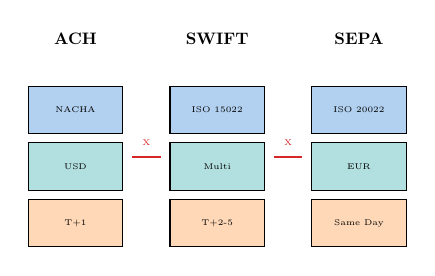
\begin{tikzpicture}[scale=0.6, transform shape]
% Protocol stack comparison
\node at (0,4) {\textbf{ACH}};
\node at (3,4) {\textbf{SWIFT}};
\node at (6,4) {\textbf{SEPA}};

% Stack boxes
\draw[fill=dfblue!30] (-1,3) rectangle (1,2);
\draw[fill=dfblue!30] (2,3) rectangle (4,2);
\draw[fill=dfblue!30] (5,3) rectangle (7,2);
\node[font=\tiny] at (0,2.5) {NACHA};
\node[font=\tiny] at (3,2.5) {ISO 15022};
\node[font=\tiny] at (6,2.5) {ISO 20022};

\draw[fill=dfteal!30] (-1,1.8) rectangle (1,0.8);
\draw[fill=dfteal!30] (2,1.8) rectangle (4,0.8);
\draw[fill=dfteal!30] (5,1.8) rectangle (7,0.8);
\node[font=\tiny] at (0,1.3) {USD};
\node[font=\tiny] at (3,1.3) {Multi};
\node[font=\tiny] at (6,1.3) {EUR};

\draw[fill=dforange!30] (-1,0.6) rectangle (1,-0.4);
\draw[fill=dforange!30] (2,0.6) rectangle (4,-0.4);
\draw[fill=dforange!30] (5,0.6) rectangle (7,-0.4);
\node[font=\tiny] at (0,0.1) {T+1};
\node[font=\tiny] at (3,0.1) {T+2-5};
\node[font=\tiny] at (6,0.1) {Same Day};

% Incompatibility symbols
\draw[thick, dfred] (1.2,1.5) -- (1.8,1.5);
\node[dfred, font=\tiny] at (1.5,1.8) {X};
\draw[thick, dfred] (4.2,1.5) -- (4.8,1.5);
\node[dfred, font=\tiny] at (4.5,1.8) {X};
\end{tikzpicture}
\end{column}
\end{columns}
\end{frame}

%--- Frame 21: Friction #6 - Limited Hours ---
\begin{frame}{Friction \#6: Limited Operating Hours}
\begin{center}
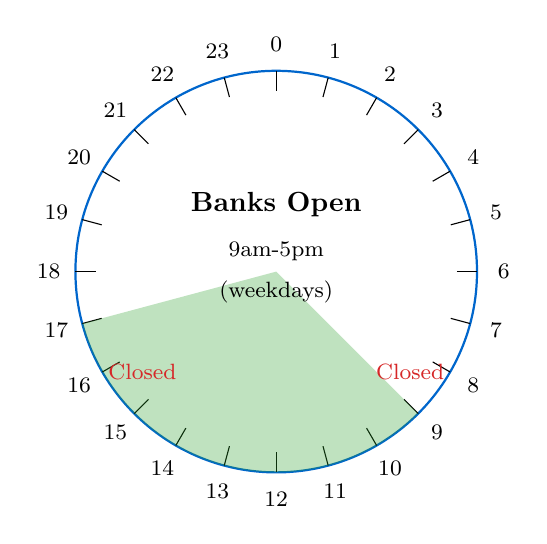
\begin{tikzpicture}[scale=0.85]
% 24-hour clock
\draw[thick, dfblue] (0,0) circle (3cm);

% Hours
\foreach \i in {0,1,...,23} {
    \draw ({90-\i*15}:2.7) -- ({90-\i*15}:3);
    \node at ({90-\i*15}:3.4) {\footnotesize \i};
}

% Business hours (shaded)
\fill[dfgreen, opacity=0.3] (0,0) -- (90-9*15:3) arc (90-9*15:90-17*15:3) -- cycle;

% Labels
\node at (0,1) {\textbf{Banks Open}};
\node at (0,0.3) {\footnotesize 9am-5pm};
\node at (0,-0.3) {\footnotesize (weekdays)};

% Night hours
\node[dfred] at (-2,-1.5) {\footnotesize Closed};
\node[dfred] at (2,-1.5) {\footnotesize Closed};
\end{tikzpicture}
\end{center}

\vspace{3mm}
\textbf{Traditional finance operates on:}
\begin{itemize}
\item Business hours only (no nights, weekends, holidays)
\item Local timezone (misaligned with global commerce)
\item Batch processing cycles (not real-time)
\end{itemize}
\end{frame}

%--- Frame 22: Limited Hours - Global Business Impact ---
\begin{frame}{Limited Hours: The Global Business Problem}
\begin{center}
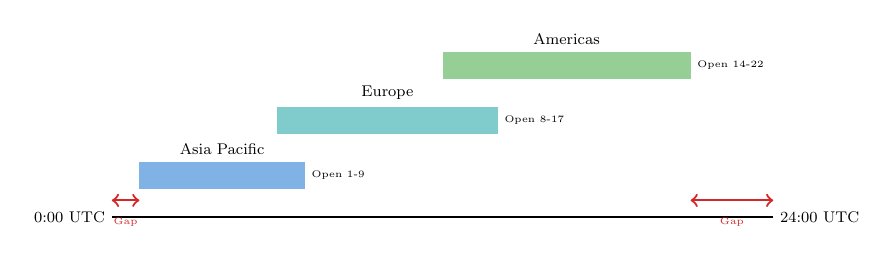
\begin{tikzpicture}[scale=0.7, transform shape]
% Timeline showing overlapping business hours
\draw[thick] (0,0) -- (12,0);
\node[left] at (0,0) {\footnotesize 0:00 UTC};
\node[right] at (12,0) {\footnotesize 24:00 UTC};

% Business hours bars
\fill[dfblue!50] (0.5,0.5) rectangle (3.5,1);
\node[above, font=\footnotesize] at (2,1) {Asia Pacific};
\node[right, font=\tiny] at (3.5,0.75) {Open 1-9};

\fill[dfteal!50] (3,1.5) rectangle (7,2);
\node[above, font=\footnotesize] at (5,2) {Europe};
\node[right, font=\tiny] at (7,1.75) {Open 8-17};

\fill[dfgreen!50] (6,2.5) rectangle (10.5,3);
\node[above, font=\footnotesize] at (8.25,3) {Americas};
\node[right, font=\tiny] at (10.5,2.75) {Open 14-22};

% Gap indicators
\draw[thick, dfred, <->] (10.5,0.3) -- (12,0.3);
\draw[thick, dfred, <->] (0,0.3) -- (0.5,0.3);
\node[below, dfred, font=\tiny] at (11.25,0.1) {Gap};
\node[below, dfred, font=\tiny] at (0.25,0.1) {Gap};
\end{tikzpicture}
\end{center}

\vspace{3mm}
\textbf{Consequences:}
\begin{itemize}
\item International transfers initiated Friday arrive Tuesday (or later)
\item Cash flow gaps force businesses to hold extra reserves
\item Time-sensitive opportunities missed during off-hours
\item Emergency financial needs unmet on weekends
\end{itemize}
\end{frame}

%--- Frame 23: Who Bears the Cost? Summary ---
\begin{frame}{Who Bears the Cost? A Summary}
\begin{center}
\renewcommand{\arraystretch}{1.4}
\begin{tabular}{|l|l|p{4.5cm}|}
\hline
\textbf{Friction} & \textbf{Primary Cost Bearer} & \textbf{Impact} \\
\hline
Slow settlement & Businesses, traders & Tied-up capital, missed opportunities \\
\hline
High fees & Consumers, migrants & Reduced purchasing power \\
\hline
Exclusion & Poor, rural, undocumented & No access to savings, credit, insurance \\
\hline
Opacity & Retail investors & Worse outcomes, exploitation \\
\hline
Fragmentation & Everyone & Inefficiency, higher costs \\
\hline
Limited hours & Global businesses & Delays, cash flow problems \\
\hline
\end{tabular}
\end{center}

\vspace{3mm}
\begin{alertblock}{Key Insight}
Friction costs are \textbf{regressive}---they hurt those with less money more than those with more.
\end{alertblock}
\end{frame}

%--- Frame 24: The Regressive Nature of Friction ---
\begin{frame}{Why Frictions Are Regressive}
\begin{columns}[T]
\begin{column}{0.48\textwidth}
\textbf{Example: \$30 Wire Transfer Fee}

\vspace{3mm}
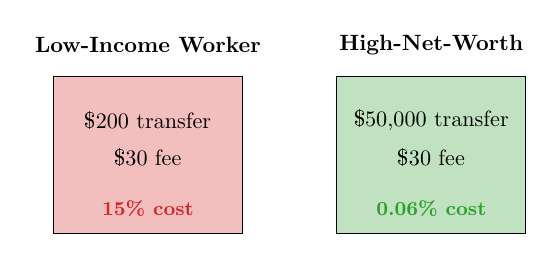
\begin{tikzpicture}[scale=0.8, transform shape]
% Two scenarios
\node at (0,3) {\textbf{Low-Income Worker}};
\draw[fill=dfred!30] (-1.5,0) rectangle (1.5,2.5);
\node at (0,1.8) {\$200 transfer};
\node at (0,1.2) {\$30 fee};
\node[dfred, font=\small] at (0,0.4) {\textbf{15\% cost}};

\node at (4.5,3) {\textbf{High-Net-Worth}};
\draw[fill=dfgreen!30] (3,0) rectangle (6,2.5);
\node at (4.5,1.8) {\$50,000 transfer};
\node at (4.5,1.2) {\$30 fee};
\node[dfgreen, font=\small] at (4.5,0.4) {\textbf{0.06\% cost}};
\end{tikzpicture}
\end{column}
\begin{column}{0.48\textwidth}
\textbf{Pattern Repeats Across All Frictions:}
\begin{itemize}
\item Minimum balances hurt those with less
\item Flat fees take larger \% from small amounts
\item Exclusion denies services to those most in need
\item Complexity favors those with advisors
\item Time delays hurt those without cushion
\end{itemize}

\vspace{3mm}
\begin{block}{Implication}
Financial innovation that reduces friction can be inherently progressive.
\end{block}
\end{column}
\end{columns}
\end{frame}

%--- Frame 25: Why Do Frictions Persist? ---
\begin{frame}{Why Do These Frictions Persist?}
\begin{columns}[T]
\begin{column}{0.48\textwidth}
\textbf{Structural Reasons:}
\begin{itemize}
\item Legacy infrastructure (COBOL systems from 1960s)
\item Regulatory requirements
\item Network effects (everyone uses existing rails)
\item High switching costs
\item Coordination problems
\end{itemize}
\end{column}
\begin{column}{0.48\textwidth}
\textbf{Incentive Reasons:}
\begin{itemize}
\item Friction = revenue for intermediaries
\item Information asymmetry benefits incumbents
\item Limited competition in some markets
\item Regulatory capture
\item ``Good enough'' for powerful customers
\end{itemize}
\end{column}
\end{columns}

\vspace{5mm}
\begin{alertblock}{Key Question}
For each friction, ask: Is this a \textbf{technical problem} or an \textbf{incentive problem}? The answer shapes the solution.
\end{alertblock}
\end{frame}

%--- Frame 26: Friction as Opportunity ---
\begin{frame}{Friction as Opportunity}
\begin{center}
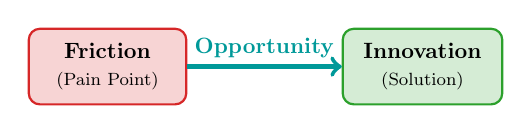
\begin{tikzpicture}[scale=0.8, transform shape, node distance=3cm]
% Friction to Innovation
\node (friction) [blockchain, minimum width=2.5cm, minimum height=1.2cm, fill=dfred!20, draw=dfred] {
\begin{tabular}{c}
\textbf{Friction}\\
\footnotesize (Pain Point)
\end{tabular}
};

\node (innovation) [blockchain, right of=friction, node distance=5cm, minimum width=2.5cm, minimum height=1.2cm, fill=dfgreen!20, draw=dfgreen] {
\begin{tabular}{c}
\textbf{Innovation}\\
\footnotesize (Solution)
\end{tabular}
};

\draw[->, ultra thick, dfteal] (friction) -- node[above] {\textbf{Opportunity}} (innovation);
\end{tikzpicture}
\end{center}

\vspace{3mm}
\begin{columns}[T]
\begin{column}{0.48\textwidth}
\textbf{Slow settlement} $\rightarrow$\\
\footnotesize Real-time payments, instant settlement

\textbf{High fees} $\rightarrow$\\
\footnotesize Low-cost transfers, crypto rails

\textbf{Exclusion} $\rightarrow$\\
\footnotesize Mobile money, neobanks
\end{column}
\begin{column}{0.48\textwidth}
\textbf{Opacity} $\rightarrow$\\
\footnotesize Transparent protocols, open data

\textbf{Fragmentation} $\rightarrow$\\
\footnotesize APIs, interoperability standards

\textbf{Limited hours} $\rightarrow$\\
\footnotesize 24/7 digital infrastructure
\end{column}
\end{columns}
\end{frame}

%--- Frame 27: Innovation Mapping ---
\begin{frame}{Mapping Frictions to Digital Finance Solutions}
\begin{center}
\footnotesize
\renewcommand{\arraystretch}{1.3}
\begin{tabular}{|l|l|l|}
\hline
\textbf{Friction} & \textbf{FinTech Solution} & \textbf{DeFi/Blockchain Solution} \\
\hline
Slow Settlement & Real-time rails (FedNow, UPI) & On-chain settlement (seconds) \\
\hline
High Fees & Wise, Remitly, neobanks & Stablecoins, L2 networks \\
\hline
Exclusion & Mobile money (M-Pesa) & Permissionless wallets \\
\hline
Opacity & Open banking APIs & Transparent smart contracts \\
\hline
Fragmentation & Plaid, Stripe, aggregators & Blockchain interoperability \\
\hline
Limited Hours & Digital-first banks & 24/7 blockchain networks \\
\hline
\end{tabular}
\end{center}

\vspace{3mm}
\begin{block}{Preview}
Topics 1.3-1.6 will explore how these solutions actually work, their trade-offs, and real-world adoption patterns.
\end{block}
\end{frame}

%--- Frame 28: Are Frictions Sometimes Features? ---
\begin{frame}{Counter-Argument: Are Some Frictions Features?}
\textbf{The Devil's Advocate Position:}

\begin{columns}[T]
\begin{column}{0.48\textwidth}
\textbf{Settlement Delay:}
\begin{itemize}
\item Time for fraud detection
\item Error correction window
\item Compliance verification
\end{itemize}

\vspace{2mm}
\textbf{Exclusion (KYC):}
\begin{itemize}
\item Anti-money laundering
\item Terrorist financing prevention
\item Consumer protection
\end{itemize}
\end{column}
\begin{column}{0.48\textwidth}
\textbf{Limited Hours:}
\begin{itemize}
\item Human oversight
\item Market stability (circuit breakers)
\item Error recovery time
\end{itemize}

\vspace{2mm}
\textbf{Opacity:}
\begin{itemize}
\item Proprietary innovation
\item Competitive differentiation
\item Security through obscurity
\end{itemize}
\end{column}
\end{columns}

\vspace{5mm}
\begin{alertblock}{Critical Thinking}
Not all friction is bad. The question is whether the friction \textbf{proportionate} to the benefit it provides.
\end{alertblock}
\end{frame}

%--- Frame 29: Discussion Questions ---
\begin{frame}{Discussion: Frictions You've Experienced}
\textbf{Think-Pair-Share:}
\begin{enumerate}
\item \textbf{Think} (2 min): Have you personally experienced any of these frictions?
\begin{itemize}
\item Waiting for a transfer?
\item Paying unexpected fees?
\item Difficulty opening an account?
\item Not understanding financial products?
\end{itemize}
\item \textbf{Pair} (3 min): Share your experience with a neighbor
\item \textbf{Share}: What patterns emerge?
\end{enumerate}

\vspace{5mm}
\begin{block}{Discussion Questions}
\begin{itemize}
\item Which friction affects you most?
\item Which friction causes the most societal harm?
\item Are any of these frictions \textit{features} rather than bugs?
\end{itemize}
\end{block}
\end{frame}

%--- Frame 30: Application Exercise ---
\begin{frame}{Application: Friction Analysis Framework}
\textbf{Use this framework to analyze any financial product or service:}

\begin{center}
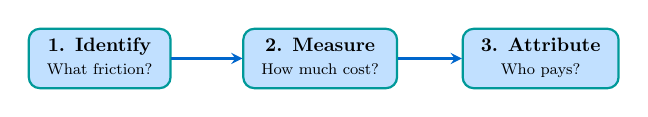
\begin{tikzpicture}[scale=0.7, transform shape]
% Framework boxes
\node (identify) [blockchain, minimum width=2.5cm] {
\begin{tabular}{c}
\textbf{1. Identify}\\
\footnotesize What friction?
\end{tabular}
};

\node (measure) [blockchain, right of=identify, node distance=4cm, minimum width=2.5cm] {
\begin{tabular}{c}
\textbf{2. Measure}\\
\footnotesize How much cost?
\end{tabular}
};

\node (who) [blockchain, right of=measure, node distance=4cm, minimum width=2.5cm] {
\begin{tabular}{c}
\textbf{3. Attribute}\\
\footnotesize Who pays?
\end{tabular}
};

\draw[arrow] (identify) -- (measure);
\draw[arrow] (measure) -- (who);
\end{tikzpicture}
\end{center}

\vspace{3mm}
\textbf{Example Analysis: International Student Tuition Payment}
\begin{itemize}
\item \textbf{Friction:} High fees (\$40-80), slow settlement (3-5 days), FX markup
\item \textbf{Cost:} 2-4\% of tuition payment
\item \textbf{Who pays:} Students and families, often from developing countries
\item \textbf{Opportunity:} Wise, Flywire, and crypto rails target this market
\end{itemize}
\end{frame}

%--- Frame 31: Executive Summary ---
\begin{frame}{Executive Summary: Key Takeaways}
\begin{block}{The Six Frictions of Traditional Finance}
\begin{enumerate}
\item \textbf{Slow Settlement:} Days to move money due to batch processing and intermediaries
\item \textbf{High Fees:} Especially for cross-border, hitting migrants hardest (\$50B+/year)
\item \textbf{Financial Exclusion:} 1.4B unbanked, 1B+ underbanked globally
\item \textbf{Opacity:} Hidden costs and information asymmetry favor institutions
\item \textbf{Fragmentation:} Incompatible systems increase costs and slow innovation
\item \textbf{Limited Hours:} 9-5 weekday banking misaligned with 24/7 global commerce
\end{enumerate}
\end{block}

\vspace{3mm}
\textbf{Core Insight:} Friction costs are \textbf{regressive}---hurting those with less money more. Every digital finance innovation targets one or more of these frictions.
\end{frame}

%--- Frame 32: Concept Map ---
\begin{frame}{Concept Map: Financial System Frictions}
\begin{center}
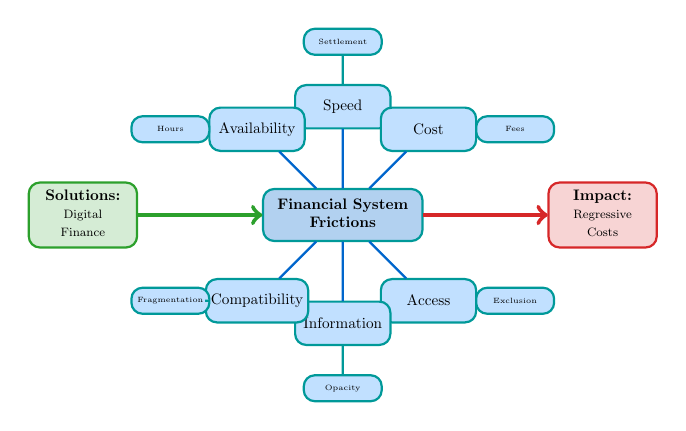
\begin{tikzpicture}[scale=0.55, transform shape]
% Central concept
\node (center) [blockchain, minimum width=3cm, minimum height=1.2cm, fill=dfblue!30] {
\begin{tabular}{c}
\textbf{Financial System}\\
\textbf{Frictions}
\end{tabular}
};

% Main friction categories
\node (speed) [blockchain, above of=center, node distance=2.5cm, minimum width=2.2cm] {Speed};
\node (cost) [blockchain, above right of=center, node distance=2.8cm, minimum width=2.2cm] {Cost};
\node (access) [blockchain, below right of=center, node distance=2.8cm, minimum width=2.2cm] {Access};
\node (info) [blockchain, below of=center, node distance=2.5cm, minimum width=2.2cm] {Information};
\node (compat) [blockchain, below left of=center, node distance=2.8cm, minimum width=2.2cm] {Compatibility};
\node (time) [blockchain, above left of=center, node distance=2.8cm, minimum width=2.2cm] {Availability};

% Connect to center
\draw[thick, dfblue] (center) -- (speed);
\draw[thick, dfblue] (center) -- (cost);
\draw[thick, dfblue] (center) -- (access);
\draw[thick, dfblue] (center) -- (info);
\draw[thick, dfblue] (center) -- (compat);
\draw[thick, dfblue] (center) -- (time);

% Sub-nodes
\node (settle) [blockchain, above of=speed, node distance=1.5cm, minimum width=1.8cm, minimum height=0.6cm, font=\tiny] {Settlement};
\node (fees) [blockchain, right of=cost, node distance=2cm, minimum width=1.8cm, minimum height=0.6cm, font=\tiny] {Fees};
\node (excl) [blockchain, right of=access, node distance=2cm, minimum width=1.8cm, minimum height=0.6cm, font=\tiny] {Exclusion};
\node (opac) [blockchain, below of=info, node distance=1.5cm, minimum width=1.8cm, minimum height=0.6cm, font=\tiny] {Opacity};
\node (frag) [blockchain, left of=compat, node distance=2cm, minimum width=1.8cm, minimum height=0.6cm, font=\tiny] {Fragmentation};
\node (hours) [blockchain, left of=time, node distance=2cm, minimum width=1.8cm, minimum height=0.6cm, font=\tiny] {Hours};

\draw[thick, dfteal] (speed) -- (settle);
\draw[thick, dfteal] (cost) -- (fees);
\draw[thick, dfteal] (access) -- (excl);
\draw[thick, dfteal] (info) -- (opac);
\draw[thick, dfteal] (compat) -- (frag);
\draw[thick, dfteal] (time) -- (hours);

% Impact node
\node (impact) [blockchain, right of=center, node distance=6cm, minimum width=2.5cm, fill=dfred!20, draw=dfred] {
\begin{tabular}{c}
\textbf{Impact:}\\
\footnotesize Regressive\\
\footnotesize Costs
\end{tabular}
};

\draw[->, ultra thick, dfred] (center) -- (impact);

% Solution node
\node (solution) [blockchain, left of=center, node distance=6cm, minimum width=2.5cm, fill=dfgreen!20, draw=dfgreen] {
\begin{tabular}{c}
\textbf{Solutions:}\\
\footnotesize Digital\\
\footnotesize Finance
\end{tabular}
};

\draw[->, ultra thick, dfgreen] (solution) -- (center);
\end{tikzpicture}
\end{center}
\end{frame}

%--- Frame 33: Key Terms (Part 1) ---
\begin{frame}{Key Terms and Definitions (Part 1)}
\begin{description}
\item[Settlement] The actual transfer of securities and/or payment between transaction parties, completing a trade.

\item[T+1 / T+2] Settlement time conventions; T+1 means settlement one business day after trade date.

\item[Correspondent Bank] An intermediary bank that provides services on behalf of another bank, often in cross-border transactions.

\item[SWIFT] Society for Worldwide Interbank Financial Telecommunication; messaging network for international payments (not settlement).

\item[Remittance] Money sent by workers to family in another country; global market exceeds \$700B annually.

\item[Unbanked] Adults without any bank account; 1.4 billion globally.

\item[Underbanked] Adults with limited access to mainstream financial services; reliant on alternatives like payday loans.
\end{description}
\end{frame}

%--- Frame 34: Key Terms (Part 2) ---
\begin{frame}{Key Terms and Definitions (Part 2)}
\begin{description}
\item[Information Asymmetry] When one party in a transaction has more relevant knowledge than the other; typically favors financial institutions.

\item[Payment for Order Flow (PFOF)] Practice where brokers receive payment for routing customer orders to market makers.

\item[Batch Processing] Processing transactions in groups at scheduled intervals rather than in real-time.

\item[Fragmentation] The existence of multiple incompatible systems requiring translation, conversion, and intermediaries to interact.

\item[Regressive Cost] A cost that takes a larger percentage from those with less money than from those with more.

\item[KYC (Know Your Customer)] Identity verification requirements imposed by financial regulations.

\item[Financial Inclusion] The availability and equality of opportunities to access useful and affordable financial services.
\end{description}
\end{frame}

%--- Frame 35: Common Misconceptions ---
\begin{frame}{Common Misconceptions}
\begin{enumerate}
\item \textbf{``Instant'' payments are actually instant}
\begin{itemize}
\item Reality: Most ``instant'' payments still have batch processing behind the scenes; actual settlement may take hours or days
\end{itemize}

\item \textbf{``Free'' services have no cost}
\begin{itemize}
\item Reality: Free trading apps monetize through payment for order flow, interest on cash, or data; you pay indirectly
\end{itemize}

\item \textbf{Financial exclusion only affects developing countries}
\begin{itemize}
\item Reality: 6\% of US adults are unbanked, 18\% underbanked; exclusion exists in all economies
\end{itemize}

\item \textbf{Digital solutions automatically reduce friction}
\begin{itemize}
\item Reality: Digital can add new frictions (e.g., digital divide, cybersecurity risks, algorithmic bias)
\end{itemize}

\item \textbf{All friction is bad and should be eliminated}
\begin{itemize}
\item Reality: Some friction provides protection (fraud detection, error correction, compliance)
\end{itemize}
\end{enumerate}
\end{frame}

%--- Frame 36: Self-Assessment Question 1 (ID: 2) ---
\begin{frame}{Self-Assessment Question 1}
\begin{block}{Question}
Approximately how many adults globally have no bank account?
\end{block}

\vspace{3mm}
\textbf{Options:}
\begin{enumerate}[A.]
\item 500 million
\item 1.4 billion
\item 3 billion
\item 5 billion
\end{enumerate}

\vspace{5mm}
\pause
\begin{alertblock}{Answer: B}
1.4 billion adults globally are unbanked, with an additional 1+ billion who are underbanked. This represents a massive financial exclusion problem where those who need financial services most have the least access to them.
\end{alertblock}
\end{frame}

%--- Frame 37: Self-Assessment Question 2 (ID: 7) ---
\begin{frame}{Self-Assessment Question 2}
\begin{block}{Question}
During what hours do traditional banks typically operate?
\end{block}

\vspace{3mm}
\textbf{Options:}
\begin{enumerate}[A.]
\item 24/7 including weekends
\item 9am-5pm weekdays only
\item 8am-8pm seven days a week
\item 6am-10pm weekdays only
\end{enumerate}

\vspace{5mm}
\pause
\begin{alertblock}{Answer: B}
Traditional banks typically operate 9am-5pm on weekdays only, creating significant friction for global commerce that operates 24/7. This limited operating schedule causes delays, cash flow problems, and misalignment with international business needs.
\end{alertblock}
\end{frame}

%--- Frame 38: Self-Assessment Question 3 (ID: 15) ---
\begin{frame}{Self-Assessment Question 3}
\begin{block}{Question}
What is the primary reason why ACH transfers take 2-3 business days despite appearing ``instant'' to users?
\end{block}

\vspace{3mm}
\textbf{Options:}
\begin{enumerate}[A.]
\item Government regulations require a waiting period
\item Banks hold funds to earn interest
\item Batch processing cycles run behind the scenes
\item Blockchain confirmation times are slow
\end{enumerate}

\vspace{5mm}
\pause
\begin{alertblock}{Answer: C}
ACH transfers take 2-3 business days because they use batch processing rather than real-time settlement. Although the user interface may show an immediate transfer, the actual movement of funds happens through scheduled batch cycles, typically processed overnight or at specific intervals.
\end{alertblock}
\end{frame}

%--- Frame 39: What's Next ---
\begin{frame}{What's Next: Topic 1.3 - Digital Solutions Overview}
\textbf{Preview of Topic 1.3:}

\begin{columns}[T]
\begin{column}{0.48\textwidth}
\textbf{We'll explore:}
\begin{itemize}
\item How FinTech addresses each friction
\item The rise of digital banking
\item Open banking and APIs
\item Mobile money revolution
\item Blockchain-based alternatives
\end{itemize}
\end{column}
\begin{column}{0.48\textwidth}
\textbf{Key questions:}
\begin{itemize}
\item Which solutions actually work?
\item What new frictions do they create?
\item Who wins and loses in the transition?
\item What role does regulation play?
\end{itemize}
\end{column}
\end{columns}

\vspace{5mm}
\begin{block}{Connection}
The pain points we studied today are the \textbf{why} behind digital finance innovation. Topic 1.3 explores the \textbf{how} and \textbf{what}.
\end{block}
\end{frame}

%--- Frame 40: Resources and Questions ---
\begin{frame}{Resources and Questions}
\textbf{Further Reading:}
\begin{itemize}
\item World Bank Global Findex Database (financial inclusion data)
\item BIS Papers on cross-border payments
\item IMF Reports on remittances
\item SWIFT Annual Review
\end{itemize}

\vspace{3mm}
\textbf{Online Resources:}
\begin{itemize}
\item Remittance Prices Worldwide: \url{remittanceprices.worldbank.org}
\item Global Findex: \url{globalfindex.worldbank.org}
\item BIS Innovation Hub: \url{bis.org/innovation}
\end{itemize}

\vspace{5mm}
\begin{center}
\LARGE Questions?
\end{center}
\end{frame}

\end{document}
